\section{Theoretical overview}
\label{sec:theory}

% In this chapter, the theoretical motivation for the study of rare decays of \B mesons is presented. Section~\ref{sec:theory:overview} gives a brief overview of the Standard Model (SM) of particle physics. Section~\ref{sec:theory:flavourviolation} describes the process of flavour violation within the SM.  The limitations of the SM are detailed in Sec.~\ref{sec:theory:limitations}. Section~\ref{sec:theory:rare} describes the decays of rare \B mesons and the effective theories used to intepret experimental measurements.

\subsection{The Standard Model of Particle Physics}
\label{sec:theory:overview}

The Standard Model of particle physics incorporates the Glashow-Weinberg-Salam theory of the electroweak interaction and quantum chromodynamics. It describes our current understanding of elementary particles and their interactions. While this section briefly describes the most relevant aspects of the SM for this thesis, a more complete description can be found in Refs.~\cite{griffiths,halzen}.

Elementary particles can be divided into two categories: fermions, with half integer spin, and bosons, with integer spin. The SM fermions consist of quarks and leptons and are often referred to as matter. The properties of the twelve SM fermions are shown in Table~\ref{tab:fermions}. The SM bosons mediate the fundamental interactions between the fermions and amongst themselves. The properties of the SM bosons are shown in Table~\ref{tab:bosons}.

\begin{table}[!b]
\def\arraystretch{1.1}
\caption{Properties of the quarks and leptons in the SM. The particle masses are taken from Ref.~\cite{pdg}.}
\begin{center}
\resizebox{\textwidth}{!}{
\begin{tabular}{ccc}
\multicolumn{3}{c}{\bf Quarks} \\
Flavour & Mass~[$\mathrm{Me\kern -0.1em V\!/}c^2$] & Charge \\
\hline
\uquark & $2.3^{+0.7}_{-0.5}$ & $+$2/3 \\
\dquark & $4.8^{+0.7}_{-0.3}$ & $-$1/3 \\
\cquark & $1275\pm25$ & $+$2/3 \\
\squark & $95\pm5$ & $-$1/3 \\
\tquark & $(160^{+5}_{-4})\times10^{3}$ & $+$2/3 \\
\bquark & $4180\pm30$ & $-$1/3 \\
\end{tabular}

\begin{tabular}{ccc}
\multicolumn{3}{c}{\bf Leptons} \\
Flavour & Mass~[$\mathrm{Me\kern -0.1em V\!/}c^2$] & Charge \\
\hline
\neue & $<2 \times 10^{-6}$ & \hphantom{$-$}0 \\
\electron & 0.510998928(11) & $-$1 \\
\neum & $<0.19$ & \hphantom{$-$}0 \\
\muon & 105.6583715(35) & $-$1 \\
\neut & $<18.2$ & \hphantom{$-$}0 \\
\tauon & 1776.86(12) & $-$1 \\
\end{tabular}
}
\end{center}
\label{tab:fermions}
\end{table}

\begin{table}[!tb]
\caption{Properties of the bosons in the SM. The particle masses are taken from Ref.~\cite{pdg}.}
\begin{center}
\resizebox{0.6\textwidth}{!}{
\begin{tabular}{lccc}
Boson & Mass~[$\mathrm{Ge\kern -0.1em V\!/}c^2$] & Charge & Spin \\
\hline 
$g$ & 0 & \hphantom{$\pm$}0 & 1 \\
\Wpm & $80.385\pm0.015\hphantom{0}$ & $\pm$1 & 1 \\
\Z & $91.187\pm0.0021$ & \hphantom{$\pm$}0 & 1 \\
$\gamma$ & 0 & \hphantom{$\pm$}0 & 1 \\
\H & $125.09\pm0.24\hphantom{00}$ & \hphantom{$\pm$}0 & 0 \\
\end{tabular}
}
\end{center}
\label{tab:bosons}
\end{table}

The SM is formulated within the framework of Quantum Field Theory (QFT) where the fermions and bosons are represented by quantum fields. The dynamics of the SM particles are described by the SM Lagrangian,

\begin{equation}
\mathcal{L}_{SM} = \mathcal{L}_{EW} + \mathcal{L}_{QCD} + \mathcal{L}_{Higgs},
\end{equation}

\noindent which is invariant under local transformations of the gauge group ${\rm SU}(3)_{C} \times {\rm SU}(2)_{L} \times {\rm U}(1)_{Y}$. The requirement of local gauge symmetry gives rise to gauge bosons corresponding to each of the symmetry groups. The ${\rm SU}(3)_{C}$ group introduces eight gluons, $g$, and represents the symmetry group of the strong interaction, resulting in the conservation of color charge, $C$. The ${\rm SU}(2)_{L} \times {\rm U}(1)_{Y}$ group introduces the \Wpm, \Z and \g bosons, and represents the symmetry group of the electroweak interaction, resulting in the conservation of weak isospin, $T$, and weak hypercharge, $Y$. 

The ${\rm SU}(2)_{L} \times {\rm U}(1)_{Y}$ symmetry is spontaneously broken by the Higgs field into the electromagnetic and weak interactions. This mechanism also generates the masses for the \Wpm and \Z bosons. The quarks and leptons obtain their masses via Yukawa couplings to the Higgs field. The fact that the Yukawa couplings are not diagonal generates the quark mixing described in Sec.~\ref{sec:theory:flavourviolation}. The Higgs boson, \H, was the final particle of the SM to be discovered when it was confirmed in 2012~\cite{higgs-atlas,higgs-cms}.

\subsection{Flavour violation in the SM}
\label{sec:theory:flavourviolation}

When only the three lightest quarks (\uquark, \dquark, \squark) were known, Cabibbo~\cite{cabbibo} proposed a mechanism to explain the observed rates of semileptonic processes. Vertices of the type $\decay{\dquark}{\uquark+\Wm}$ were given a factor $\cos\theta_{C}$, while those of the type $\decay{\squark}{\uquark+\Wm}$ were given a factor $\sin\theta_{C}$, where $\theta_{C}\sim13^{\circ}$ is the Cabibbo angle. This mechanism was found to be very successful in describing many decay rates but there was a problem: it allowed the \Kz meson to decay into a \mumu pair. The amplitude of this process should be proportional to $\sin\theta_{C}\cos\theta_{C}$ but the calculated rate was much greater than the experimental limit. 

A solution was proposed by Glashow, Iliopoulos and Maini (GIM)~\cite{gim} who introduced the fourth quark, \cquark, with vertex couplings of $-\sin\theta_{C}$ and $\cos\theta_{C}$ for $\decay{\dquark}{\cquark+\Wm}$ and $\decay{\squark}{\cquark+\Wm}$ transitions respectively. This was several years before the \cquark quark was observed experimentally~\cite{jpsi-1,jpsi-2}. According to the GIM mechanism, the diagram for the decay \decay{\Kz}{\mumu} in Fig.~\ref{fig:ktomm:a} is almost exactly cancelled by the corresponding diagram in Fig.~\ref{fig:ktomm:b} with a virtual \cquark quark replacing the \uquark. The small rate that remains is due to the differences in the masses of the \uquark quark and the \cquark quark.

\begin{figure}[!tb]
\centering
\begin{subfigure}{0.49\textwidth}
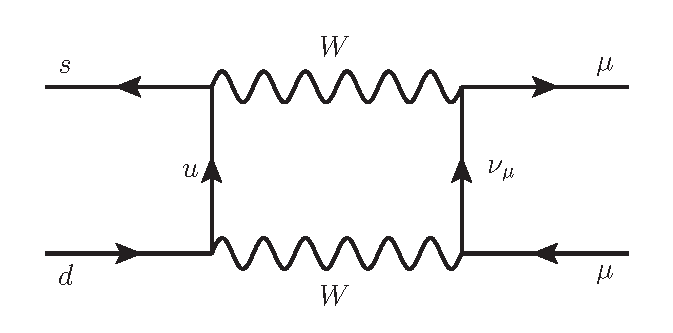
\includegraphics[width=\linewidth]{figs/theory/KToMuMu_uquark.eps}
\caption{}
\label{fig:ktomm:a}
\end{subfigure}
\begin{subfigure}{0.49\textwidth}
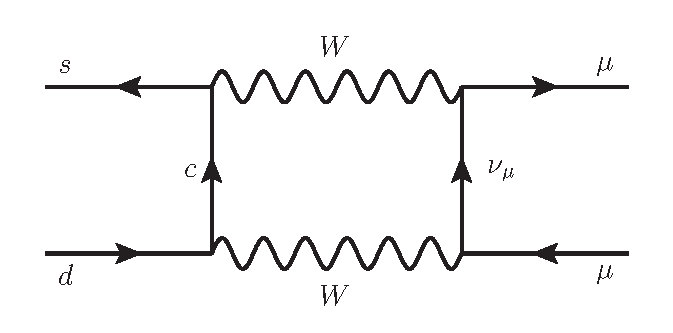
\includegraphics[width=\linewidth]{figs/theory/KToMuMu_cquark.eps}
\caption{}
\label{fig:ktomm:b}
\end{subfigure}
\caption{Feynman diagrams contributing to the decay \decay{\Kz}{\mumu}. The amplitude for each diagram is proportional to the product of the coupling at each vertex: (a) $\sin\theta_{C}\cos\theta_{C}$, (b)  $-\sin\theta_{C}\cos\theta_{C}$. The total amplitude is found by summing the two contributions.}
\label{fig:ktomm}
\end{figure}

In the Cabibbo-GIM scheme, it can be intepreted that the \W does not couple to the mass eigenstates \dquark and \squark but instead to the weak eigenstates $\dquark^\prime$ and $\squark^\prime$, given by

\begin{equation}
\dquark^\prime = \dquark\cos\theta_{C}+\squark\sin\theta_{C},~~~\squark^\prime = -\dquark\sin\theta_{C}+\squark\cos\theta_{C}
\end{equation}

\noindent or in `Cabibbo matrix' form

\begin{equation}
\binom{\dquark^\prime}{\squark^\prime} = 
\begin{pmatrix}
\cos\theta_{C} & \sin\theta_{C} \\
-\sin\theta_{C} & \cos\theta_{C} \\
\end{pmatrix}
\binom{\dquark}{\squark}.
\end{equation}

Even before the discovery of the \cquark quark, Kobayaski and Maskawa~\cite{kobayashi-maskawa} had generalised the Cabibbo-GIM scheme to incorporate three generations of quarks. This was motivated by the desire to explain \CP violation within the Cabibbo-GIM scheme, which was not possible with only two generations. The weak eigenstates are related to the mass eigenstates through the CKM matrix

\begin{equation}
\begin{pmatrix}
\dquark^\prime \\
\squark^\prime \\
\bquark^\prime \\
\end{pmatrix}
=
\begin{pmatrix}
\Vud & \Vus & \Vub \\
\Vcd & \Vcs & \Vcb \\
\Vtd & \Vts & \Vtb \\
\end{pmatrix}
\begin{pmatrix}
\dquark \\
\squark \\
\bquark \\
\end{pmatrix}
\end{equation}

\noindent where each matrix element, \Vij, specifies the coupling of $i$ to $j$. The additional generation of quarks increases the number of free parameters from one ($\theta_{C}$) to four: three `generalised Cabibbo angles' ($\theta_{12}$, $\theta_{23}$, $\theta_{13}$) and a complex phase $\delta$. This complex phase generates \CP violation in the quark sector. 

\subsection{Beyond the SM}
\label{sec:theory:limitations}

Despite its considerable success in predicting cross-sections and branching ratios of particles with great accuracy, the SM it is not without its limitations, some of which are outlined below

\begin{itemize}
  \item Gravity, the fourth fundamental force, is not incorporated in the SM. However, this is not specific to the SM as there is no consensus on how to include gravity in a QFT. 
  \item The SM has 19 free parameters: the 9 fermion masses, the 4 parameters of the CKM matrix, 3 gauge coupling constants, the Higgs vacuum expectation value $v$, the Higgs quartic coupling $\lambda$ and the QCD $\theta$ parameter. 
  \item Dark matter, which is believed to be five times as abundant as ordinary matter, is not accounted for in the SM.
  \item The amount of \CP violation predicted by the SM is ten orders of magnitude lower than what is needed to account for the observed matter-antimatter asymmetry in the Universe, assuming matter and antimatter were created in equal amounts in the Big Bang.
  \item The measured mass of the Higgs boson implies a large cancellation between the bare mass and quantum corrections. The nature of a mechanism that could provide a natural cancellation of these corrections is unknown.
\end{itemize}

\noindent These limitations have led physicists to look for extensions to the SM in the form of New Physics (NP) models. Such NP models often predict new particles that may contribute to, and therefore modify, flavour-changing processes in the SM.

\subsection{Rare decays of \B mesons}
\label{sec:theory:rare}

Flavour-changing neutral current (FCNC) transitions are forbidden at tree level in the SM. They are rare processes that occur via loop and box diagrams, making them an ideal place to perform a search for NP. Rare decays of \B mesons, such as those containing a \btosll transition, can have sizeable NP contributions that are not swamped by the competing SM process. 

By studying the properties of FCNC processes it is possible to perform model independent searches sensitive to a wide range of NP models. Feyman diagrams for the \btosll transition, both in the SM and in possible NP scenarios~\cite{Gauld:2013qja,Altmannshofer:2014cfa,Crivellin:2015mga}, are shown Fig.~\ref{fig:btosll}. New particles can modify the dynamics of a decay: changing the branching fraction or the kinematic distribution of the final state particles. By comparing the SM prediction of observables with experimental measurements, the flavour structure of NP models can be probed. The theoretical framework used to interpret flavour physics measurements in a model independent way is the so-called Operator Product Expansion (OPE)~\cite{ope}.

\begin{figure}[!tb]
\centering
\begin{subfigure}{0.49\textwidth}
\begin{tikzpicture}
\node[anchor=south west,inner sep=0](image) at (0,0) {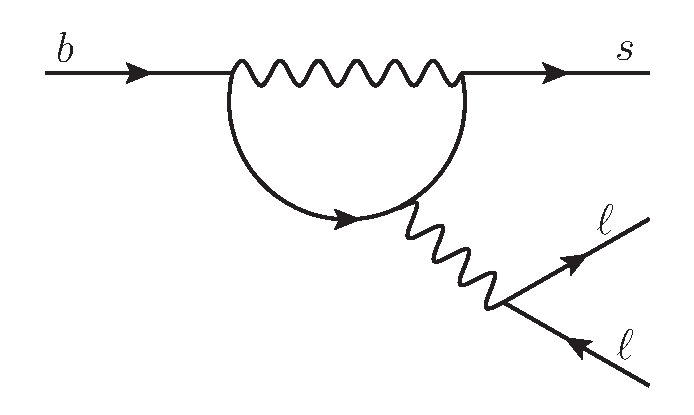
\includegraphics[width=\textwidth]{figs/theory/btosll_penguin.eps}};
\begin{scope}[x={(image.south east)},y={(image.north west)}]
%\draw[help lines,xstep=.1,ystep=.1] (0,0) grid (1,1);
\node[draw=none,bleudefrance] at (0.53,0.96) {\small \Wm};
\node[draw=none,bleudefrance] at (0.3,0.6) {\small \tquark};
\node[draw=none,bleudefrance] at (0.56,0.27) {\small \Pgamma, $\Z^{0}$};
\node[draw=none,bleudefrance] at (0.2,0.2) {SM};
\end{scope}
\end{tikzpicture}
\caption{}
\label{fig:btosll:a}
\end{subfigure}
\begin{subfigure}{0.49\textwidth}
\begin{tikzpicture}
\node[anchor=south west,inner sep=0](image) at (0,0) {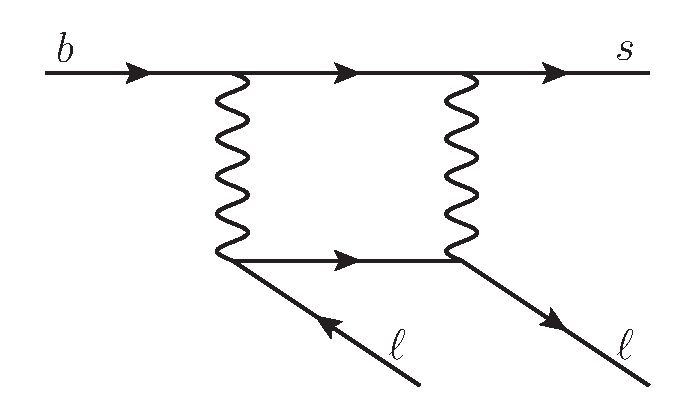
\includegraphics[width=\textwidth]{figs/theory/btosll_box.eps}};
\begin{scope}[x={(image.south east)},y={(image.north west)}]
%\draw[help lines,xstep=.1,ystep=.1] (0,0) grid (1,1);
\node[draw=none,bleudefrance] at (0.5,0.95) {\small \tquark};
\node[draw=none,bleudefrance] at (0.25,0.6) {\small \Wm};
\node[draw=none,bleudefrance] at (0.8,0.6) {\small \Wp};
\node[draw=none,bleudefrance] at (0.5,0.45) {\small \Pnu};
\node[draw=none,bleudefrance] at (0.2,0.2) {SM};
\end{scope}
\end{tikzpicture}
\caption{}
\label{fig:btosll:b}
\end{subfigure}
\begin{subfigure}{0.49\textwidth}
\begin{tikzpicture}
\node[anchor=south west,inner sep=0](image) at (0,0) {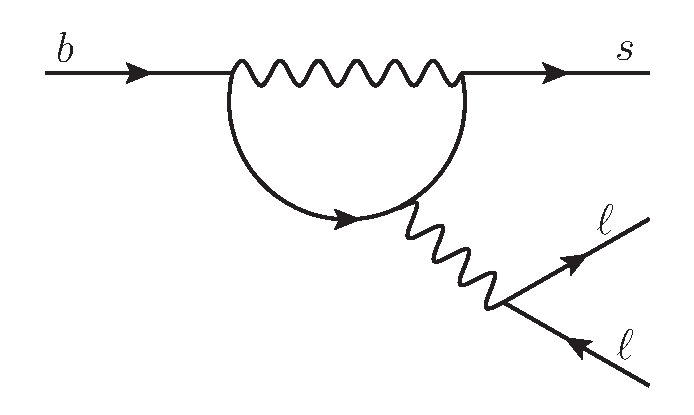
\includegraphics[width=\textwidth]{figs/theory/btosll_penguin.eps}};
\begin{scope}[x={(image.south east)},y={(image.north west)}]
%\draw[help lines,xstep=.1,ystep=.1] (0,0) grid (1,1);
\node[draw=none,bostonuniversityred] at (0.5,0.96) {\small $\tilde{g}$};
\node[draw=none,bostonuniversityred] at (0.3,0.6) {\small $\tilde{d}_{i}$};
\node[draw=none,bostonuniversityred] at (0.58,0.27) {\small $\H$};
\node[draw=none,bostonuniversityred] at (0.2,0.2) {NP};
\end{scope}
\end{tikzpicture}
\caption{}
\label{fig:btosll:c}
\end{subfigure}
\begin{subfigure}{0.49\textwidth}
\begin{tikzpicture}
\node[anchor=south west,inner sep=0](image) at (0,0) {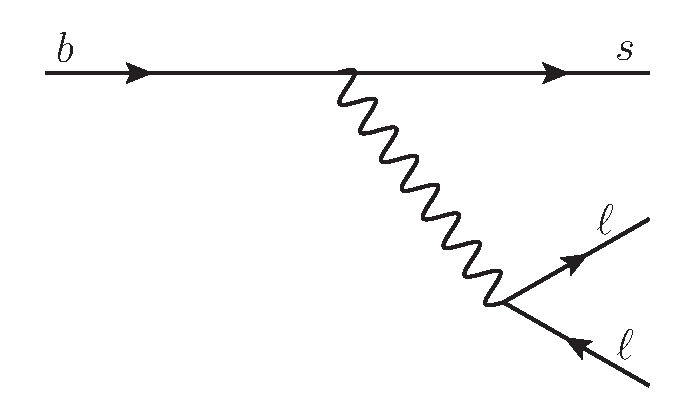
\includegraphics[width=\textwidth]{figs/theory/btosll_zprime.eps}};
\begin{scope}[x={(image.south east)},y={(image.north west)}]
%\draw[help lines,xstep=.1,ystep=.1] (0,0) grid (1,1);
\node[draw=none,bostonuniversityred] at (0.55,0.45) {\small $Z^{'}$};
\node[draw=none,bostonuniversityred] at (0.2,0.2) {NP};
\end{scope}
\end{tikzpicture}
\caption{}
\label{fig:btosll:d}
\end{subfigure}
\caption{Feynman diagrams for the FCNC transition \btosll: in the SM (a,b) and in possible NP scenarios (c,d).}
\label{fig:btosll}
\end{figure}

In the OPE approach, all degrees of freedom above a given energy scale, $\Lambda$, are integrated out. This is valid as long as $\Lambda$ is much larger than the energy scale of the decay, $\mu$, which for the study of \B mesons is chosen to be $\order(m_{\bquark})$. This formalism is analogous to Fermi's effective theory of weak decay in which the full theory is reduced to a four point interaction, as shown in Fig.~\ref{fig:beta} for $\beta$-decay.

\begin{figure}[!tb]
\centering
\begin{subfigure}{0.49\textwidth}
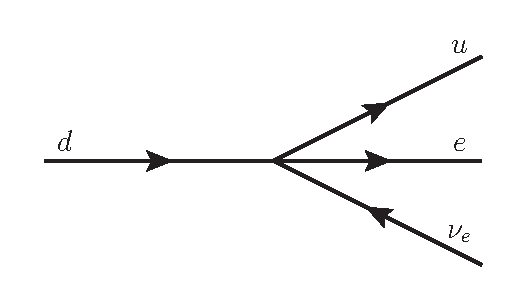
\includegraphics[width=\linewidth]{figs/theory/beta_4point.eps}
\caption{}
\label{fig:beta:a}
\end{subfigure}
\begin{subfigure}{0.49\textwidth}
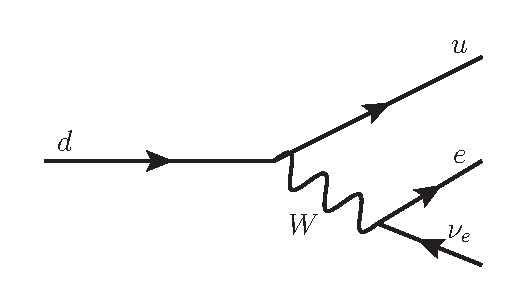
\includegraphics[width=\linewidth]{figs/theory/beta_w.eps}
\caption{} 
\label{fig:beta:b}
\end{subfigure}
\caption{Feynman diagrams for $\beta$-decay in the (a) effective theory and (b) full theory.}
\label{fig:beta}
\end{figure}

In the SM, the effective Hamiltonian describing \btosll decays can be written as

\begin{equation}
\mathcal{H}_{\rm eff} = - \frac{4G_{F}}{\sqrt{2}}V_{tb}V^{*}_{ts}\sum_{i}[\mathcal{C}_{i}(\mu)\mathcal{O}_{i}(\mu) + \mathcal{C}^{'}_{i}(\mu)\mathcal{O}^{'}_{i}(\mu)].
\end{equation}

\noindent where $G_{F}$ is the Fermi constant, and $V_{ij}$ are CKM matrix elements. The complex Wilson coefficients, $\mathcal{C}_{i}$, incorporate the short distance (high energy) contributions. For each Wilson coefficient, there is a local operator $\mathcal{O}_{i}$ which incorporates the long distance (low energy) contributions. The primed operators represent the right-handed currents, which are highly suppressed in the SM. The advantage of the OPE approach is that the Wilson coefficients are independent of the underlying process and can include contributions from NP. 

For \btosll decays, the dominant contributions in the SM arise from the following operators~\cite{operators}

\begin{alignat}{2}
&\order_{7} = \frac{e}{g^{2}}m_{\bquark}(\squarkbar\sigma_{\mu\nu}P_{R}\bquark)F^{\mu\nu},~~~~~&&\order_{7}^{\prime} = \frac{e}{g^{2}}m_{\bquark}(\squarkbar\sigma_{\mu\nu}P_{L}\bquark)F^{\mu\nu}, \nonumber \\
&\order_{9} = \frac{e^{2}}{g^{2}}(\squarkbar\gamma_{\mu}P_{L}\bquark)(\ellbar\gamma^{\mu}\ell), &&\order_{9}^{\prime} = \frac{e^{2}}{g^{2}}(\squarkbar\gamma_{\mu}P_{R}\bquark)(\ellbar\gamma^{\mu}\ell), \nonumber \\
&\order_{10} = \frac{e^{2}}{g^{2}}(\squarkbar\gamma_{\mu}P_{L}\bquark)(\ellbar\gamma^{\mu}\gamma_{5}\ell), &&\order_{10}^{\prime} = \frac{e^{2}}{g^{2}}(\squarkbar\gamma_{\mu}P_{R}\bquark)(\ellbar\gamma^{\mu}\gamma_{5}\ell), \\
&\order_{S} = \frac{e^{2}}{16\pi^{2}}m_{\bquark}(\squarkbar P_{R}\bquark)(\ellbar\ell), &&\order_{S}^{\prime} = \frac{e^{2}}{16\pi^{2}}m_{\bquark}(\squarkbar P_{L}\bquark)(\ellbar\ell), \nonumber\\
&\order_{P} = \frac{e^{2}}{16\pi^{2}}m_{\bquark}(\squarkbar P_{R}\bquark)(\ellbar\gamma_{5}\ell), &&\order_{P}^{\prime} = \frac{e^{2}}{16\pi^{2}}m_{\bquark}(\squarkbar P_{L}\bquark)(\ellbar\gamma_{5}\ell), \nonumber
\end{alignat}

\noindent where $P_{L/R} = (1\mp\gamma_{5})/2$ are the left- and right-handed projection operators. The operator $\order_{7}$ is the electromagnetic operator corresponding to the emission of a photon. The vector and axial-vector operators, $\order_{9}$ and $\order_{10}$, describe the $Z$ penguin and $W$ box diagrams. The operators $\order_{S}$ and $\order_{P}$ represent scalar and pseudoscalar operators.

